\documentclass[12pt]{report}
\usepackage{graphicx}
\usepackage{float}
\begin{document}

\paragraph{Project:} NanoLab Evaporator Quartz Crystal Monitor
\paragraph{Goal:} To create a quartz crystal monitor for a low-cost evaporator. It will monitor the thickness of metal that has been evaporated to control the process. 

\paragraph{Engineering Work:}
We will be using the standard quartz crystals for this project from Inficon. The main challenge is finding a way to hold the crystal so that it can still vibrate and connect to the electrical contacts. The monitor also needs to be able to adjust the angle so that it can aim directly at the source to limit shadowing and simplify the calibration for deposited material. \\
To make the electrical contact to the chip, we need to hold only the very edge of the front surface and make a spring contact on the back to keep it pressed in place. The most common way to do this is with leaf springs. We also need to ensure the two sides are electrically separated. \\
We made two copper plates on either side of a Teflon spacer. One plate held the front of the crystal, while the other had a cut-out so that a block with the leaf spring attached could slide in, twist under some tabs, and lock in place. The two plates are so thin that they could not be tapped. Instead they were bolted together so that the space on the opposite plate where they would have touched was cut away. 
$$
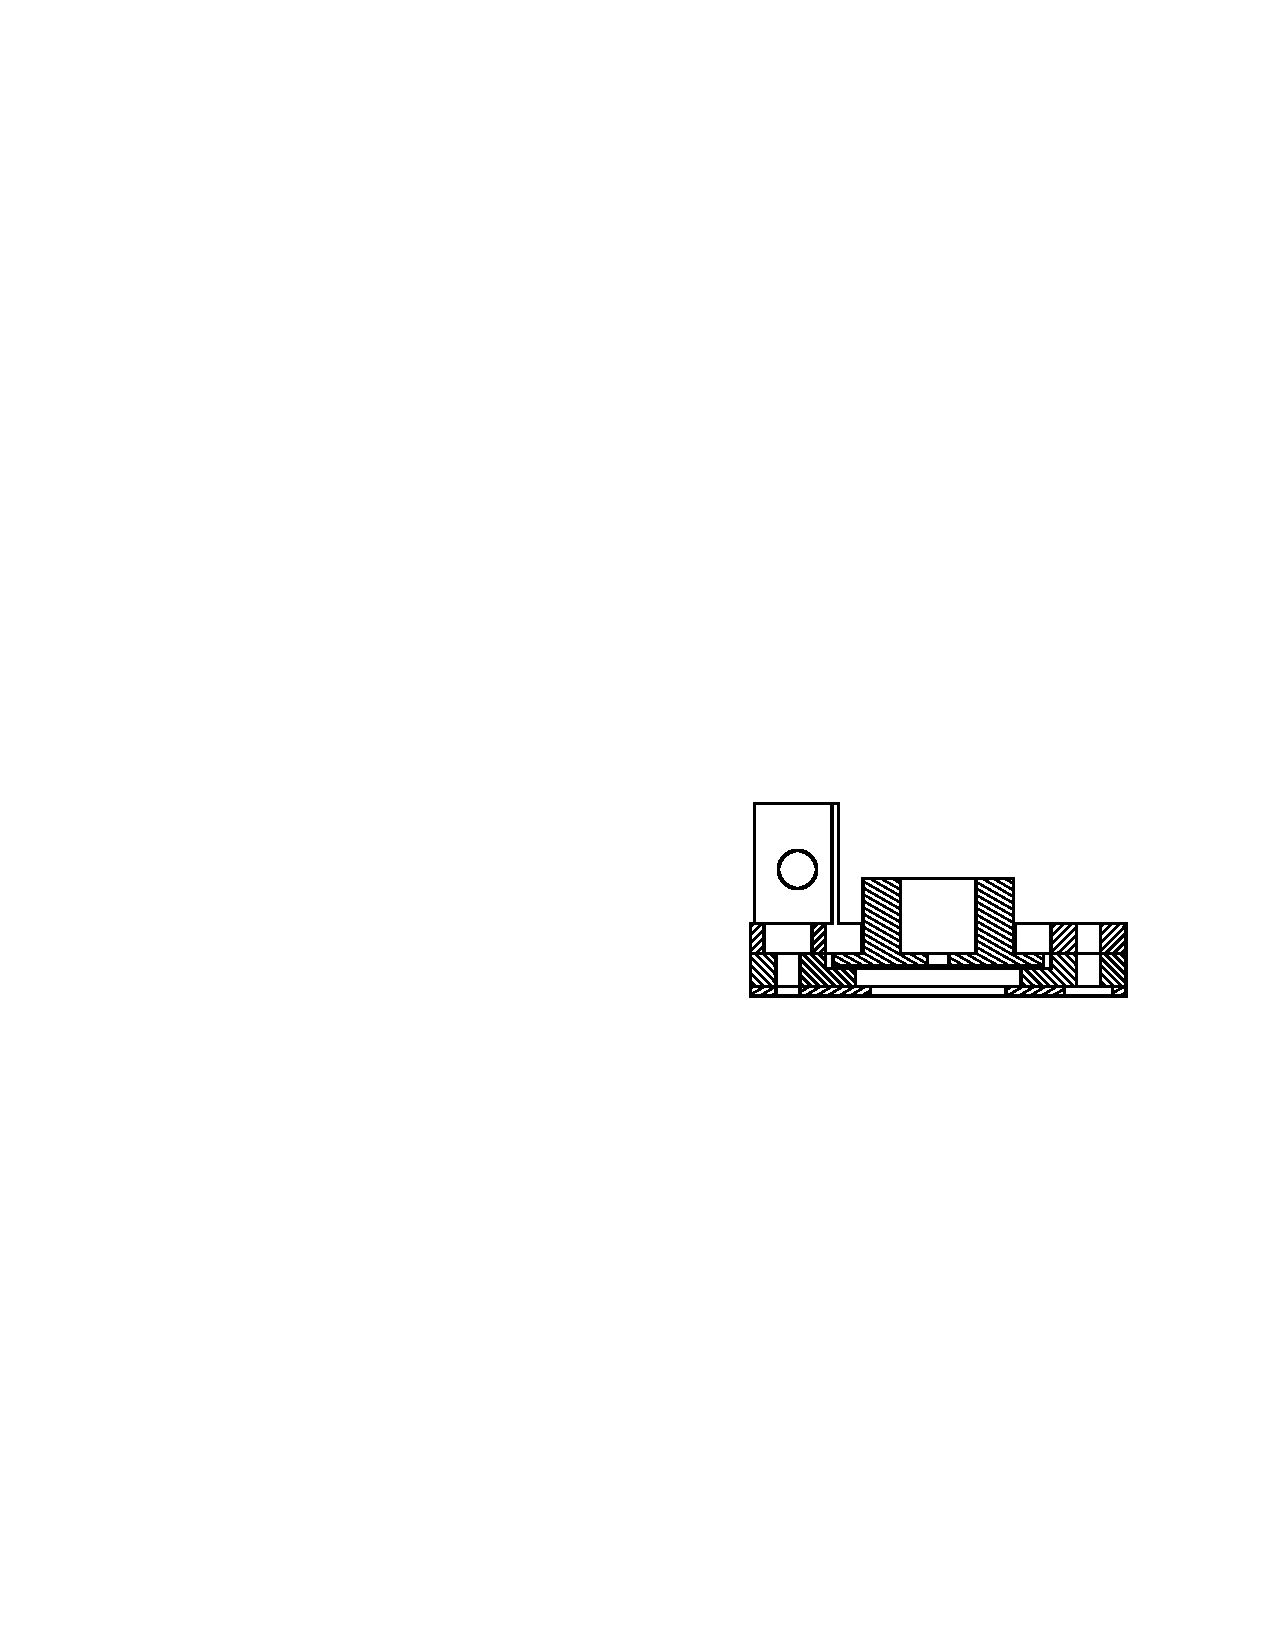
\includegraphics[scale = 0.7]{fig1}
$$
In this figure, notice the difference in diameter on the clearance holes for the bolts. Also, notice the tabs sticking out of the spring holder. This next figure shows the space for those tabs to rotate under on the top plate. 
$$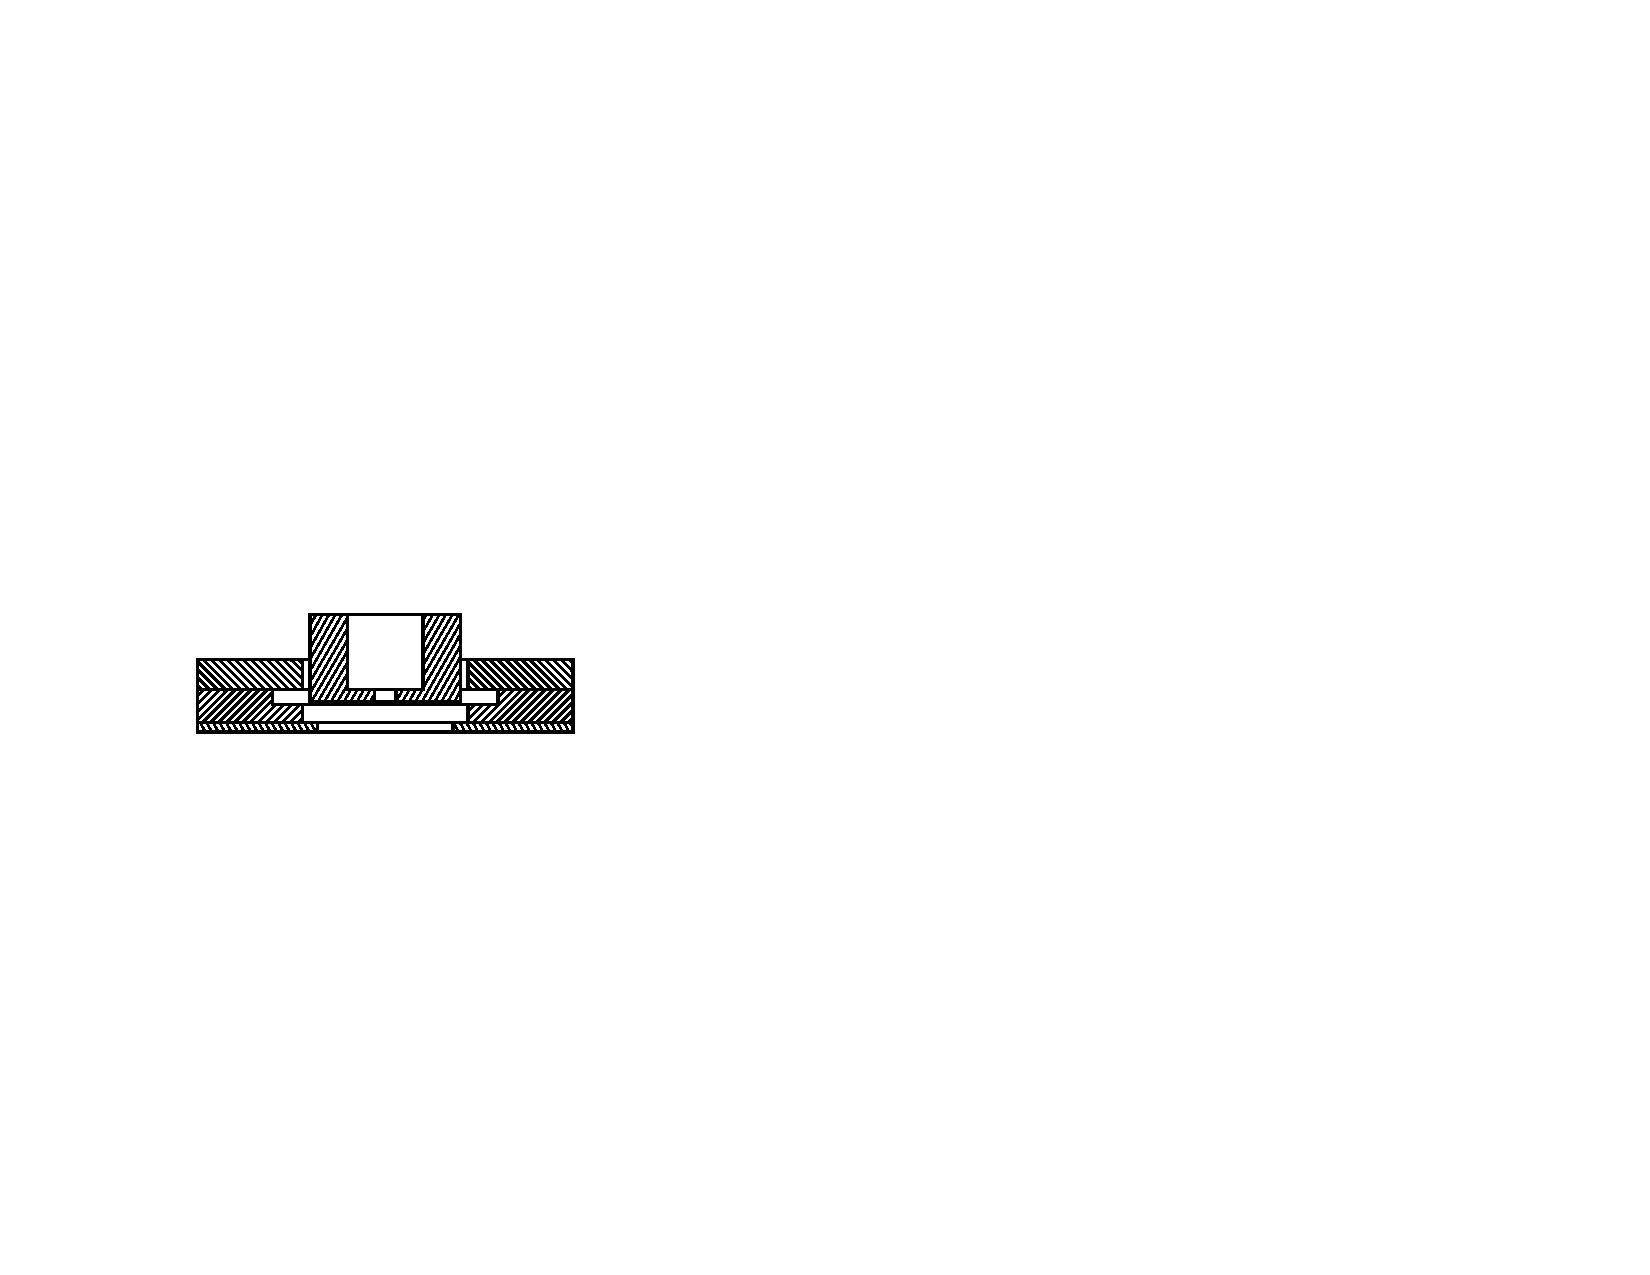
\includegraphics{fig2}$$
$$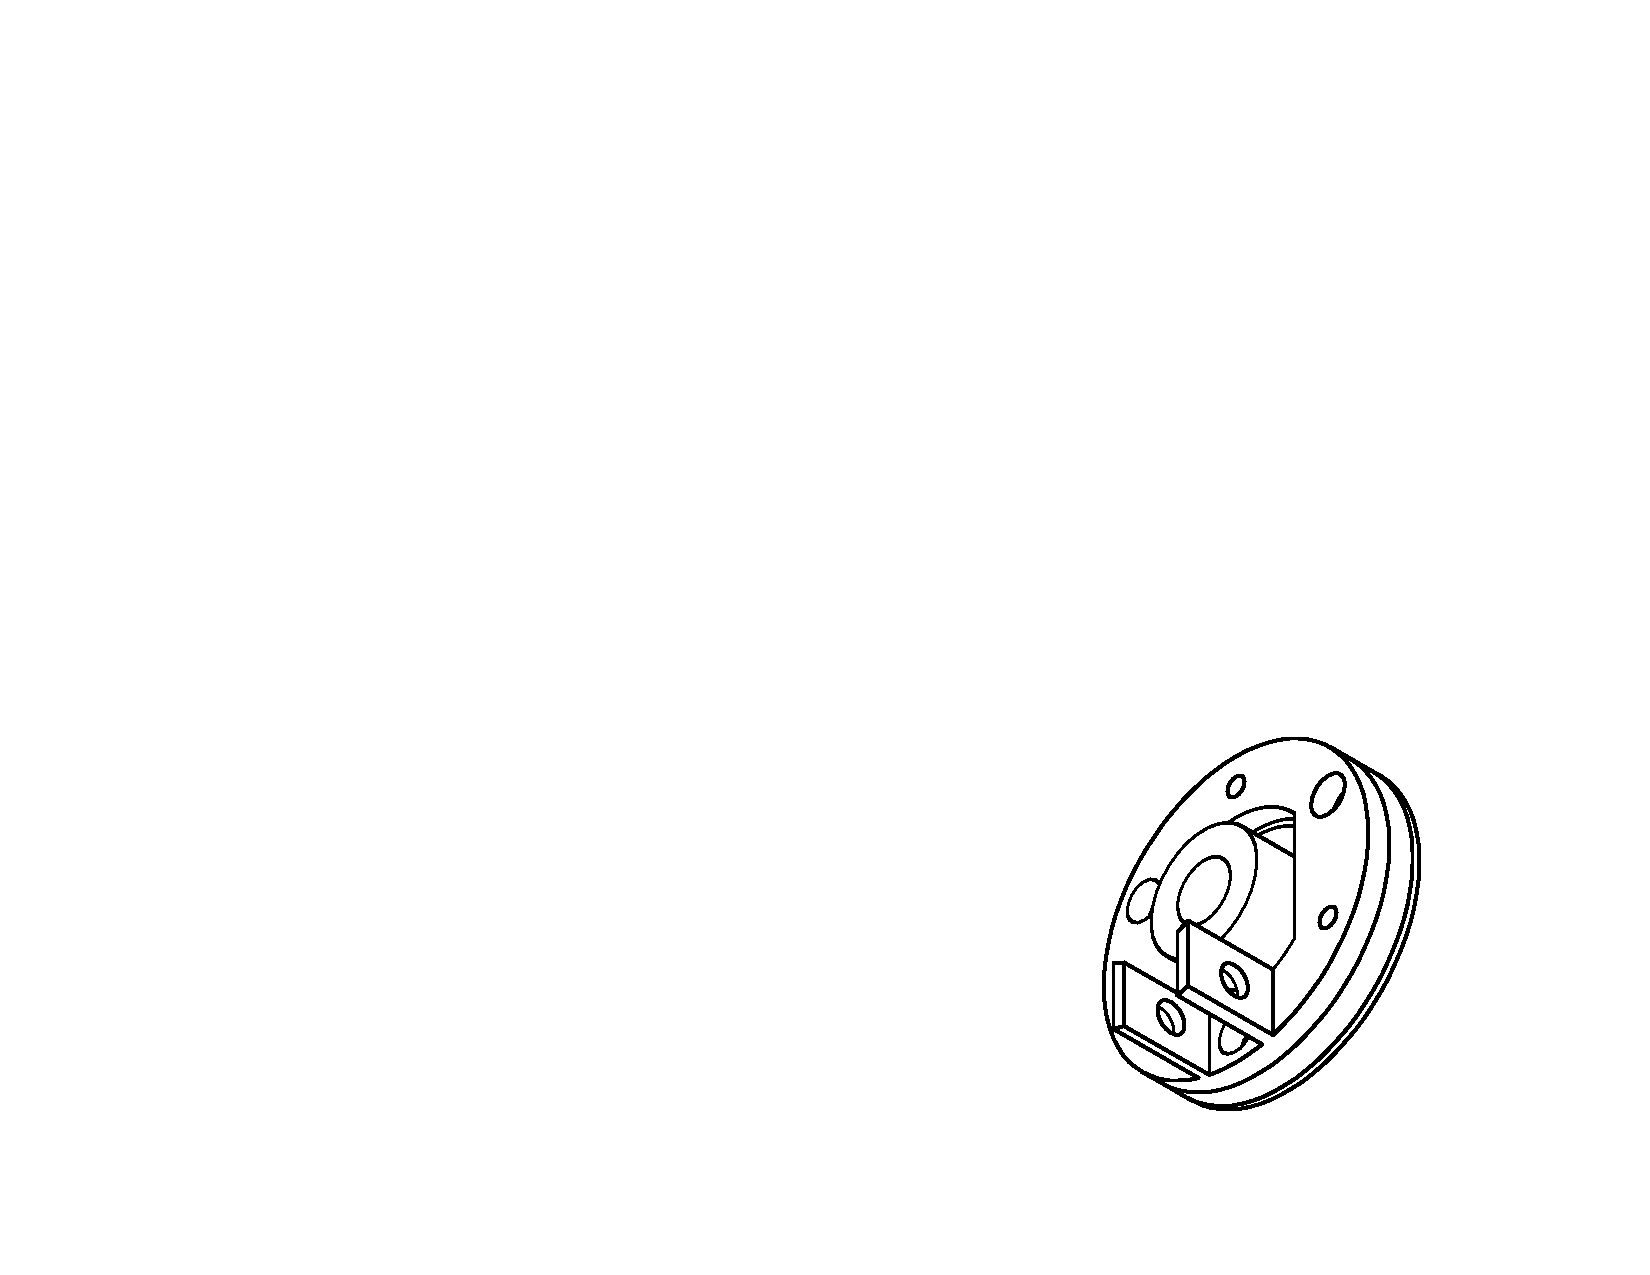
\includegraphics[scale=0.9]{fig3}$$
The last figure shows an isometric view of the whole piece. The two posts sticking out of one side are for attaching the holder to a mounting post. This post is pretty simple - it is an aluminum rod threaded on one end that is screwed into a hole in a blank flange. The threaded section has a hole drilled out of the center to relieve the gas trapped in the hole when the chamber is evacuated. The other side of the rod is drilled out to hold a rod connected to the monitor. this allows the length of the whole mounting post to be adjusted. For more details see the 3D files attached.\\
We ran into a few issues while machining the pieces. The bottom plate was made from thin copper sheet, but the upper piece had to be milled from copper rod. The stock was not wide enough, so we had to shrink some dimensions for this prototype. We cut the sides off - overall this should not affect the performance of the piece. Also, the Teflon spacer was not wide enough to hold the crystal, so it had to be sanded wider. This may have made the hole for the crystal off-center, because the crystal didn't sit perfectly in the center of the bottom copper plate. This could also be due to the crystal slipping in between the Teflon and copper - it is thin enough to do that. \\
We also ran into issues with electrical isolation. The two plates are separated, but it is pretty finicky and takes some fiddling. Also, in order to keep the whole monitor system isolated from the capacitance of the entire evaporator, we had to use Teflon washers and a Teflon screw to hold the monitor to the mounting post. In the future, the shorter telescoping section of the post should be made from a non-conducting material to isolate the system.

\paragraph{Components List:} \hspace{1cm} \\
\begin{tabular}{c|c|c}
Part & Number/Requirements & Supplier\\
\hline
Copper Sheet & 0.031" Thick, 1.25" Square & -\\
Teflon Sheet & 1/8" Thick, 1.25" Square & -\\
Copper Rod & 1/2" x 1.25" x 12" & -\\
Leaf Spring & - & -\\
Screws & 6 @ 1-72 x 1/2", 1 @ 0-80 x 1/2" & -\\
Teflon Screw, Washers & M3 x 16mm & -\\

\end{tabular}



\end{document}
